% --------------------------------------------------------------------------------

\begin{exercise}[Exercise 3.14]

The Bellman equation \eqref{eq:2.14} must hold for each state for the value function $v_\pi$ shown in Figure \ref{fig:2.14} (right). %of Example 3.5.
Show numerically that this equation holds for the center state, valued at $+0.7$, with respect to its four neighboring states, valued at $+2.3$, $+0.4$, $-0.4$, and $+0.7$.
(These numbers are accurate only to one decimal place.)

\begin{figure}[H]
    \centering
    \subfloat
    {
        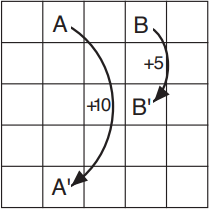
\includegraphics[width = 0.2 \textwidth]{2.14.1.png}
    }
    \hspace{1cm}
    \subfloat
    {
        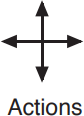
\includegraphics[width = 0.075 \textwidth]{2.14.2.png}
    }
    \hspace{1cm}
    \subfloat
    {
        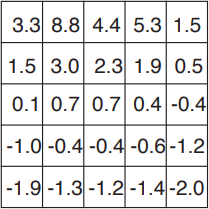
\includegraphics[width = 0.2 \textwidth]{2.14.3.png}
    }
    \hspace{0mm}
    \caption
    {
        Gridworld example:
        exceptional reward dynamics (left) and state-value function for the equiprobable random policy (right).
    }
    \label{fig:2.14}
\end{figure}

\begin{align} \label{eq:2.14}
    v_\pi(s)
    \doteq
    \sum_a
        \pi(a \mid s)
        \sum_{s^\prime, r}
            p(s^\prime, r \mid s, a)
            \bbraces{r + \gamma v_\pi(s^\prime)},
    \quad
    ~\text{for all}~ s \in \mathcal S
\end{align}

\end{exercise}

% --------------------------------------------------------------------------------

\begin{solution}

Let $s$ denote the center state.

\begin{align*}
    &
    \sum_{a \in \mathcal A(s)}
        \pi(a \mid s)
        \sum_{\substack{s^\prime \in \mathcal S \\ r \in \mathcal R}}
            p(s^\prime, r \mid s, a)
            [r + \gamma v_\pi(s^\prime)] \\
    & \approx
    \frac{1}{4} \cdot (1 \cdot (0 + 0.9 \cdot 2.3))
    +
    \frac{1}{4} \cdot (1 \cdot (0 + 0.9 \cdot 0.4))
    +
    \frac{1}{4} \cdot (1 \cdot (0 + 0.9 \cdot (-0.4)))
    +
    \frac{1}{4} \cdot (1 \cdot (0 + 0.9 \cdot 0.7)) \\
    & =
    \frac{1}{4} \cdot 0.9 \cdot (2.3 - 0.4 + 0.4 + 0.7) \\
    & =
    0.675 \\
    & \approx
    0.7 \\
    & =
    v_\pi(s)
\end{align*}

\end{solution}

% --------------------------------------------------------------------------------
